% =========================================================
% Các style TikZ dùng chung cho cả báo cáo
% =========================================================
\tikzset{
  block/.style     = {draw, rectangle, rounded corners=3pt, minimum width=2.2cm, minimum height=0.85cm, align=center, fill=blue!10, draw=blue!60, font=\small},
  io/.style        = {draw, trapezium, trapezium left angle=75, trapezium right angle=105, minimum width=2cm, minimum height=0.8cm, align=center, fill=green!10, draw=green!60!black, font=\small},
  decision/.style  = {draw, diamond, aspect=2.2, minimum width=2cm, minimum height=0.7cm, align=center, fill=orange!15, draw=orange!70, font=\scriptsize},
  arrow/.style     = {-{Stealth[length=2mm]}, draw=gray!70, thick},
  sarrow/.style    = {-{Stealth[length=2mm]}, draw=blue!50, thick, dashed},
  bus/.style       = {draw, rectangle, minimum width=4cm, minimum height=0.5cm, fill=gray!20, draw=gray!60, font=\tiny},
  chip/.style      = {draw, rectangle, rounded corners=2pt, minimum width=3cm, minimum height=1.2cm, align=center, fill=yellow!15, draw=orange!60, font=\small\bfseries},
  fpga/.style      = {draw, rectangle, rounded corners=5pt, minimum width=5.5cm, minimum height=3.5cm, align=center, fill=blue!5, draw=blue!50, very thick},
  signal/.style    = {draw=red!70, thick},
}

% =========================================================
% LAB 3  -  I2C Master Controller
% =========================================================
\newpage
\setcounter{section}{2}
\section{LAB3: DEVELOP SOFTWARE FOR NIOS II - PROCESSOR WITH SDRAM}

\subsection{Trình bày, vẽ sơ đồ mạch theo cách hiểu của học viên}

LAB3 tập trung vào thiết kế hệ thống SoC sử dụng vi xử lý Nios II kết hợp với bộ nhớ SDRAM để lưu trữ dữ liệu và mã lệnh. Sơ đồ mạch bên dưới thể hiện hệ thống được xây dựng trên Qsys/Platform Designer bao gồm bộ điều khiển SDRAM, JTAG UART, và các PIO I/O dùng để điều khiển LED/nút nhấn:

\begin{figure}[H]
    \centering
    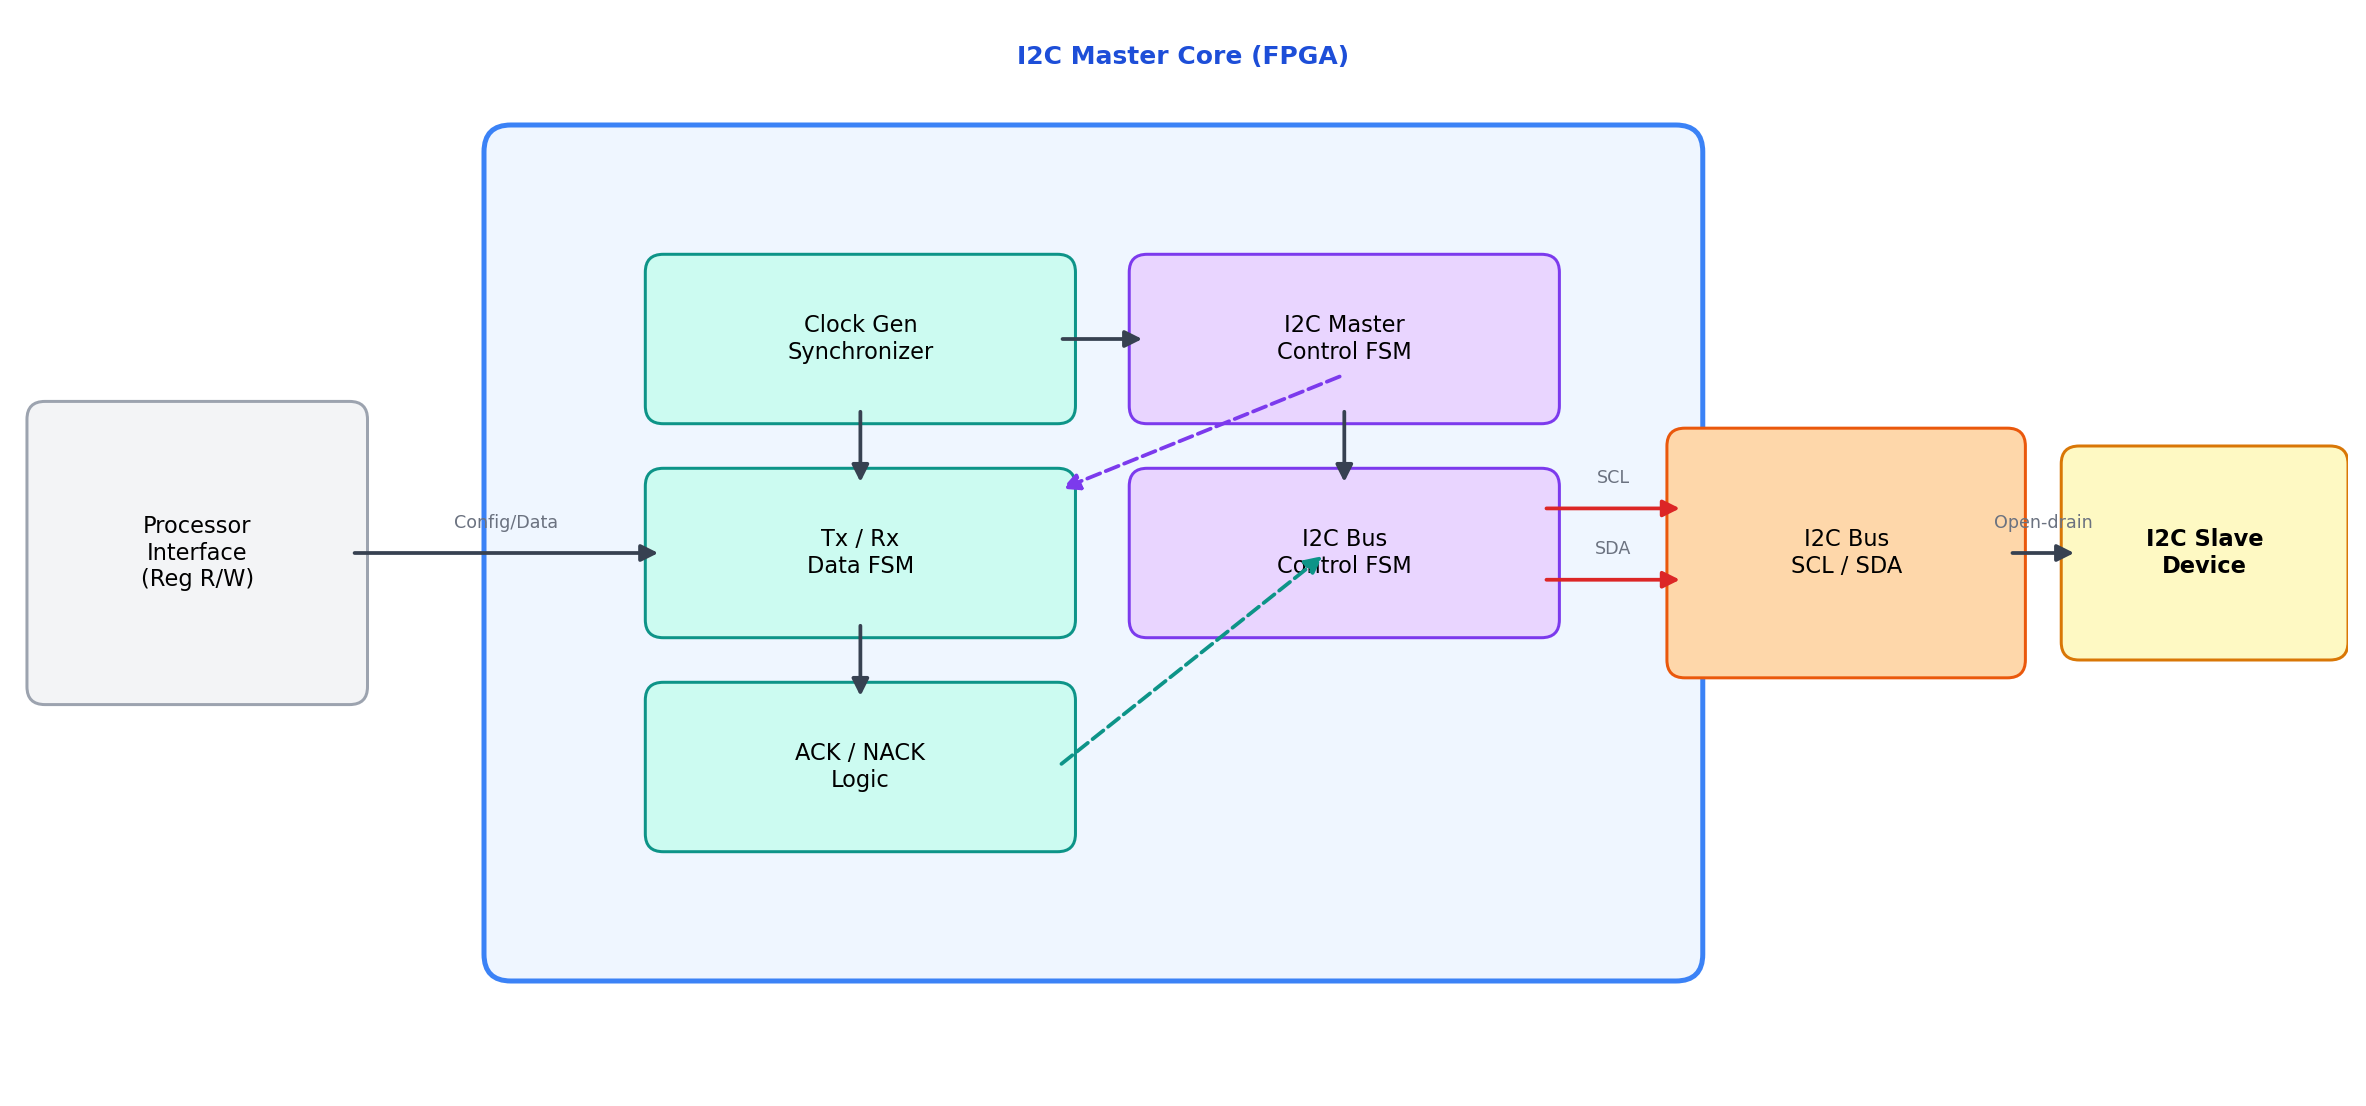
\includegraphics[width=\linewidth]{images/fig_4_1.png}
    \caption{Sơ đồ kiến trúc kết nối hệ thống Nios II với SDRAM và PIO (LAB3)}
\end{figure}

\subsection{Sơ đồ dataflow với code software}

\begin{figure}[H]
    \centering
    \begin{tikzpicture}[node distance=0.8cm]
        \node[io]                               (start)  {Bắt đầu chương trình};
        \node[block, below=of start]            (initA)  {Tạo mảng A ngẫu nhiên\\(10 phần tử)};
        \node[block, below=of initA]            (copy)   {Sao chép mảng A\\sang mảng B};
        \node[block, below=of copy]             (sort)   {Sắp xếp mảng B\\(Bubble Sort)};
        \node[block, below=of sort]             (printA) {In mảng A (chưa sắp xếp)\\ra Console};
        \node[block, below=of printA]           (printB) {In mảng B (đã sắp xếp)\\ra Console};
        \node[io, below=of printB]              (end)    {Kết thúc};

        \draw[arrow] (start)  -- (initA);
        \draw[arrow] (initA)  -- (copy);
        \draw[arrow] (copy)   -- (sort);
        \draw[arrow] (sort)   -- (printA);
        \draw[arrow] (printA) -- (printB);
        \draw[arrow] (printB) -- (end);
    \end{tikzpicture}
    \caption{Sơ đồ dataflow thuật toán sắp xếp mảng SDRAM - LAB3}
\end{figure}

Đoạn mã C minh họa chương trình sắp xếp mảng:
\begin{lstlisting}[language=C, caption={C Source Code - LAB3}]
#include <stdio.h>
#include <stdlib.h>
#include <time.h>
#include <inttypes.h>
#define SIZE 10
int main () {
int A[SIZE];

int B[SIZE];
srand(time(NULL));
for (int i = 0; i < SIZE; i++) {
// rand() % (max - min + 1) + min -> Range from [-1000:1000]
A[i] = rand() % (2001) - 1000;
}
// Copy A to B
for (int i = 0; i < SIZE; i++) {
B[i] = A[i];
}
// bubble sort
for (int i = 0; i < SIZE - 1; i++) {
for (int j = 0; j < SIZE - i - 1; j++) {
if (B[j] > B[j + 1]) {
int temp = B[j];
B[j] = B[j + 1];
B[j + 1] = temp;
}
}
}
// In A
printf("Array A (original):\n");
for (int i = 0; i < SIZE; i++) {
printf("A[%d] = %" PRId16 "\n", i, A[i]);
}
// In B
printf("\nArray B (sorted):\n");
for (int i = 0; i < SIZE; i++) {
printf("B[%d] = %" PRId16 "\n", i, B[i]);
}
return 0;
}
\end{lstlisting}

\subsection{Báo cáo kết quả Quartus synthesis implementation, resource, $f_{max}$}
Kết quả synthesis Resource và $f_{max}$ của LAB3:

\begin{figure}[H]
    \centering
    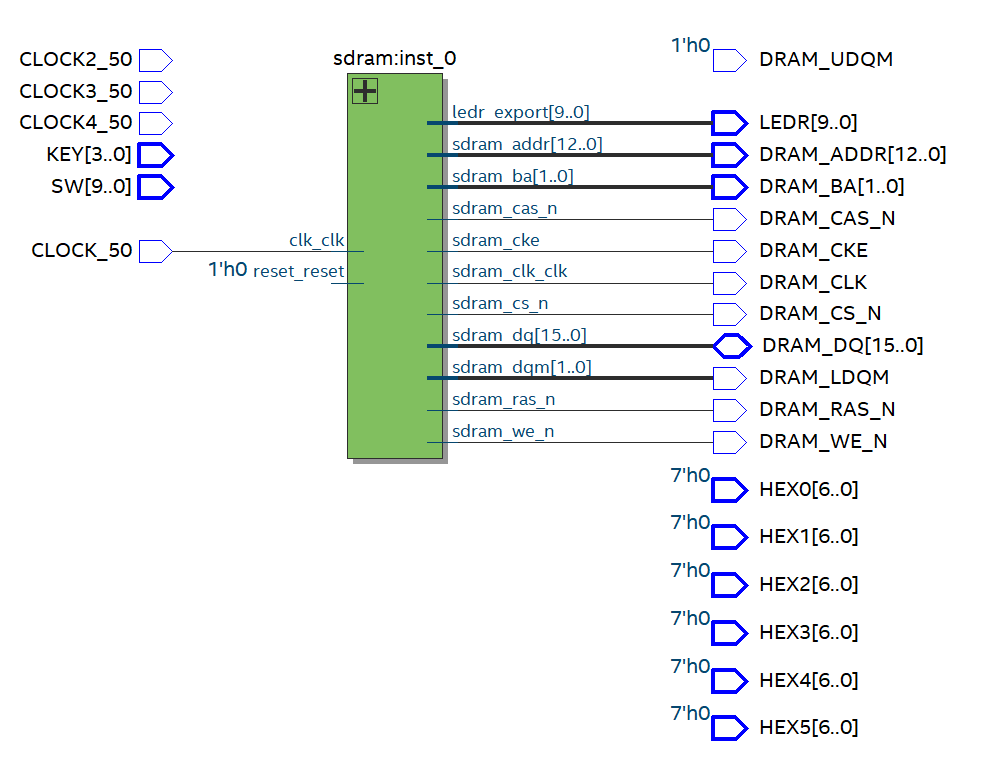
\includegraphics[width=0.9\linewidth]{images/lab3_rtl_view_new_0.png}
    \caption{RTL View của LAB3 (Cập nhật)}
\end{figure}

\begin{figure}[H]
    \centering
    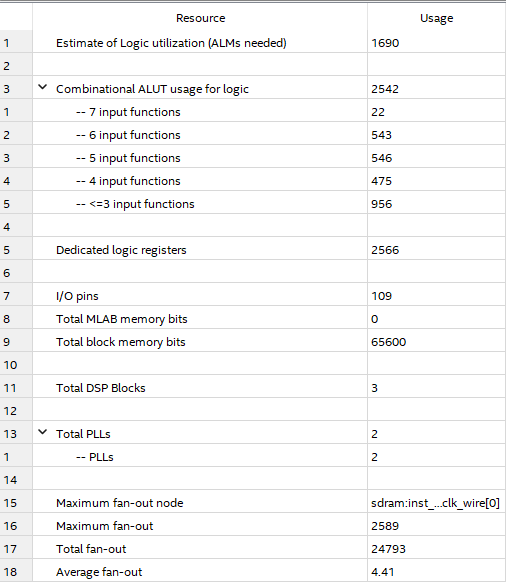
\includegraphics[width=0.9\linewidth]{images/lab3_resource.png}
    \caption{Tài nguyên sử dụng (Resource) của LAB3}
\end{figure}

\begin{figure}[H]
    \centering
    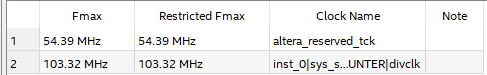
\includegraphics[width=0.9\linewidth]{images/lab3_fmax.png}
    \caption{Tần số hoạt động tối đa ($f_{max}$) của LAB3}
\end{figure}

\subsection{Hình ảnh chạy test code trên console}
Dưới đây là kết quả thực thi chương trình trên Nios II Console:
\begin{figure}[H]
    \centering
    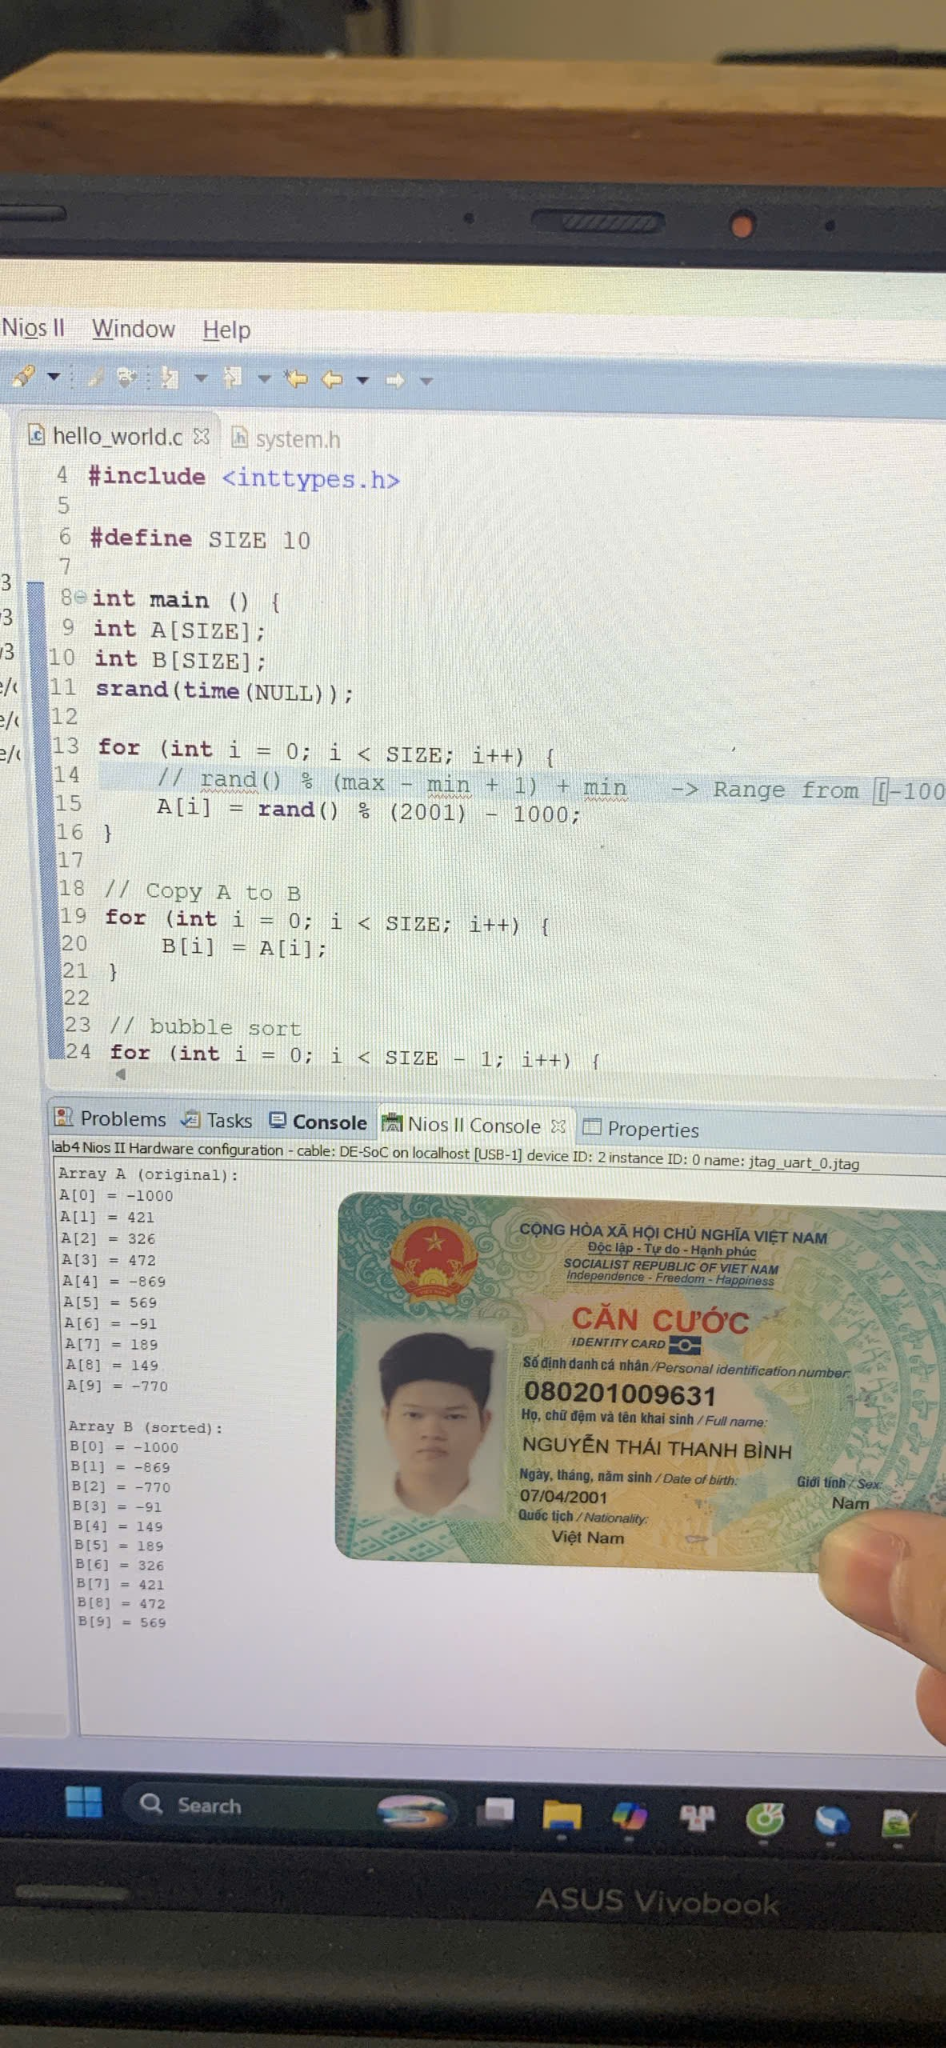
\includegraphics[width=0.8\textwidth]{images/lab3_console_0.png}
    \caption{Kết quả chạy test code trên console (LAB3)}
\end{figure}


% =========================================================
% LAB 4 & 5
% =========================================================
\newpage
\section{LAB4 \& 5: DEVELOP SOFTWARE FOR NIOS II - PROCESSOR WITH TIMER}

\subsection{Trình bày, vẽ sơ đồ mạch theo cách hiểu của học viên}

\begin{figure}[H]
    \centering
    \begin{tikzpicture}[node distance=1.5cm, auto]
        \node[chip, fill=orange!20] (nios) {Nios II Processor};
        \node[bus, minimum width=10cm, below=of nios] (avalon) {Avalon-MM System Interconnect Fabric};
        
        \node[chip, fill=green!20, below=of avalon, xshift=-3cm] (timer) {Timer IP};
        \node[chip, fill=red!20, below=of avalon, xshift=0cm] (pio_sw) {PIO (Switches)};
        \node[chip, fill=red!20, below=of avalon, xshift=3cm] (pio_led) {PIO (LEDs)};
        
        \draw[sarrow, <->] (nios.south) -- (avalon.north -| nios.south);
        \draw[sarrow, <->] (avalon.south -| timer.north) -- (timer.north);
        \draw[sarrow, <->] (avalon.south -| pio_sw.north) -- (pio_sw.north);
        \draw[sarrow, <->] (avalon.south -| pio_led.north) -- (pio_led.north);
        
        \node[io, below=of pio_sw] (sw) {Hardware Switches};
        \node[io, below=of pio_led] (led) {Hardware LEDs};
        
        \draw[signal, ->] (sw.north) -- (pio_sw.south);
        \draw[signal, ->] (pio_led.south) -- (led.north);
    \end{tikzpicture}
    \caption{Sơ đồ kiến trúc kết nối hệ thống Nios II với Timer và PIO (LAB 4 \& 5)}
\end{figure}

\subsection{Sơ đồ dataflow với code software}

\begin{figure}[H]
    \centering
    \begin{tikzpicture}[node distance=0.8cm and 1cm]
        \node[io] (start) {Bắt đầu};
        \node[block, below=of start] (init) {Khởi tạo Alarm \& cấu hình I/O};
        \node[block, below=of init] (loop) {Vòng lặp chính (while 1)};
        \node[decision, below=of loop] (read_sw) {Đọc Switch};
        
        \node[block, left=of read_sw, xshift=-2cm] (sw_03) {Bật tất cả LED};
        \node[block, right=of read_sw, xshift=2cm] (sw_00) {Tắt tất cả LED};
        
        \node[block, below=of read_sw, yshift=-1cm] (wait) {Chờ Alarm Callback ngắt};
        \node[decision, below=of wait] (cb) {Callback nào?};
        
        \node[block, below left=of cb, xshift=-0.5cm] (cb_even) {Nháy LED chẵn/lẻ};
        \node[block, below right=of cb, xshift=0.5cm] (cb_sw) {Nháy LED 1-5/6-10};
        
        \draw[arrow] (start) -- (init);
        \draw[arrow] (init) -- (loop);
        \draw[arrow] (loop) -- (read_sw);
        
        \draw[arrow] (read_sw) -- node[above] {SW=0x03} (sw_03);
        \draw[arrow] (read_sw) -- node[above] {SW=0x00} (sw_00);
        \draw[arrow] (read_sw) -- node[right] {SW=0x01, 0x02} (wait);
        
        \draw[arrow] (sw_03) |- (loop);
        \draw[arrow] (sw_00) |- (loop);
        
        \draw[arrow] (wait) -- (cb);
        \draw[arrow] (cb) -- node[above left] {Alarm chẵn/lẻ} (cb_even);
        \draw[arrow] (cb) -- node[above right] {Alarm 1-5/6-10} (cb_sw);
        
        \draw[arrow] (cb_even.south) -- ++(0,-0.5) -| (loop.west);
        \draw[arrow] (cb_sw.south) -- ++(0,-0.5) -| (loop.east);
        
    \end{tikzpicture}
    \caption{Sơ đồ dataflow thuật toán điều khiển LED bằng Timer (LAB 4 \& 5 - Exercise 3)}
\end{figure}

\subsubsection{Exercise 1}

Đoạn mã C cho Exercise 1:
\begin{lstlisting}[language=C, caption={C Source Code - LAB4\&5 Exercise 1}]
#include <stdio.h>
#include <alt_types.h>
#include <sys/alt_alarm.h>
#include "system.h"
#include "altera_avalon_pio_regs.h"
// Define BASE address
#define LED_BASE 0x04081050
#define SW_BASE 0x04081040
static alt_alarm alarm;

static int control = 0x01;
alt_u32 led_alarm_callback(void* context) {
IOWR_ALTERA_AVALON_PIO_DATA(LED_BASE, control);
control = control << 1 | 0x01;
if (control == 2047) { // 0x11111111111
control = 0x00;
}
// Return tick for 500ms
return alt_ticks_per_second() / 2;
}
int main() {
if (alt_alarm_start(&alarm, alt_ticks_per_second() / 2, led_alarm_callback,
NULL) < 0) {
printf("No system clock available\n");
return -1;
}
while (1) {
}
return 0;
}
\end{lstlisting}

\subsubsection{Exercise 2}

Đoạn mã C cho Exercise 2:
\begin{lstlisting}[language=C, caption={C Source Code - LAB4\&5 Exercise 2}]
#include <stdio.h>
#include <alt_types.h>
#include <sys/alt_alarm.h>
#include "system.h"
#include "altera_avalon_pio_regs.h"
// Define BASE address
#define LED_BASE 0x04081050
#define SW_BASE 0x04081040

static alt_alarm alarm1, alarm3, alarm5, alarm7, alarm9;
static int led_state[10] = {0};
static int is_SW1_SET = 0;
void set_led(int index, int state) {
if (is_SW1_SET == 1) {
int mask = (1 << index);
int current = IORD_ALTERA_AVALON_PIO_DATA(LED_BASE);
if (state)
current |= mask;
else
current &= ~mask;
IOWR_ALTERA_AVALON_PIO_DATA(LED_BASE, current);
led_state[index] = state;
}
else {
IOWR_ALTERA_AVALON_PIO_DATA(LED_BASE, 0x00); // OFF
all LED
for (int i = 0; i < 10; i++) led_state[i] = 0;
}
}
alt_u32 cb_led1(void* context) {
set_led(0, !led_state[0]); // LED1
return alt_ticks_per_second() * 2; // 0.25Hz = 4s
}
alt_u32 cb_led3(void* context) {
set_led(2, !led_state[2]); // LED3
return alt_ticks_per_second() * 1; // 0.5Hz = 2s
}
alt_u32 cb_led5(void* context) {
set_led(4, !led_state[4]); // LED5
return alt_ticks_per_second() / 2; // 1Hz = 1s
}
alt_u32 cb_led7(void* context) {
set_led(6, !led_state[6]); // LED7
return alt_ticks_per_second() / 4; // 2Hz = 0.5s
}
alt_u32 cb_led9(void* context) {
set_led(8, !led_state[8]); // LED9

return alt_ticks_per_second() / 8; // 4Hz = 0.25s
}
int main() {
IOWR_ALTERA_AVALON_PIO_DATA(LED_BASE, 0x00);
alt_alarm_start(&alarm1, alt_ticks_per_second() * 2, cb_led1, NULL);
alt_alarm_start(&alarm3, alt_ticks_per_second() * 1, cb_led3, NULL);
alt_alarm_start(&alarm5, alt_ticks_per_second() / 2, cb_led5, NULL);
alt_alarm_start(&alarm7, alt_ticks_per_second() / 4, cb_led7, NULL);
alt_alarm_start(&alarm9, alt_ticks_per_second() / 8, cb_led9, NULL);
while (1) {
if (IORD_ALTERA_AVALON_PIO_DATA(SW_BASE) == 0x01){
is_SW1_SET = 1;
}
else {
is_SW1_SET = 0;
}
}
return 0;
}
\end{lstlisting}

\subsubsection{Exercise 3}

Đoạn mã C cho Exercise 3:
\begin{lstlisting}[language=C, caption={C Source Code - LAB4\&5 Exercise 3}]
#include <stdio.h>
#include <alt_types.h>
#include <sys/alt_alarm.h>
#include "system.h"
#include "altera_avalon_pio_regs.h"
// Define BASE address
#define LED_BASE 0x04081050
#define SW_BASE 0x04081040
static alt_alarm alarm_even, alarm_odd, alarm_sw1_5, alarm_sw6_10;

static int led_state[10] = {0};
static int even_step = 0;
static int odd_step = 0;
static int sw1_5_step = 0;
static int sw6_10_step = 0;
void set_led(int index, int state) {
int mask = 1 << index;
int current = IORD_ALTERA_AVALON_PIO_DATA(LED_BASE);
if (state)
current |= mask; // bật LED
else
current &= ~mask; // tắt LED
IOWR_ALTERA_AVALON_PIO_DATA(LED_BASE, current);
led_state[index] = state;
}
alt_u32 cb_even(void* context) {
if (IORD_ALTERA_AVALON_PIO_DATA(SW_BASE) == 0x01) {
if (even_step == 5) {
even_step = 0;
int current = IORD_ALTERA_AVALON_PIO_DATA(LED_BASE);
int mask = (1<<1) | (1<<3) | (1<<5) | (1<<7) | (1<<9);
current &= ~mask; // Set 0 for even led
IOWR_ALTERA_AVALON_PIO_DATA(LED_BASE, current);
} else {
int led_index = (even_step * 2) + 1; // 1,3,5,7,9 → LED2,4,6,8,10
set_led(led_index, 1);
even_step++;
}
}
return alt_ticks_per_second() / 2; // 500ms
}
alt_u32 cb_odd(void* context) {
if (IORD_ALTERA_AVALON_PIO_DATA(SW_BASE) == 0x01) {
if (odd_step == 5) {

odd_step = 0;
int current = IORD_ALTERA_AVALON_PIO_DATA(LED_BASE);
int mask = (1<<0) | (1<<2) | (1<<4) | (1<<6) | (1<<8);
current &= ~mask; // Set 0 for odd led
IOWR_ALTERA_AVALON_PIO_DATA(LED_BASE, current);
} else {
int led_index = (odd_step * 2); // 0,2,4,6,8 → LED1,3,5,7,9
set_led(led_index, 1);
odd_step++;
}
}
return alt_ticks_per_second(); // 1s
}
alt_u32 cb_sw1_5(void* context) {
if (IORD_ALTERA_AVALON_PIO_DATA(SW_BASE) == 0x02) {
if (sw1_5_step == 5) {
sw1_5_step = 0;
int current = IORD_ALTERA_AVALON_PIO_DATA(LED_BASE);
int mask = (1<<0) | (1<<1) | (1<<2) | (1<<3) | (1<<4);
current &= ~mask; // Set 0 for LED 1 - 5
IOWR_ALTERA_AVALON_PIO_DATA(LED_BASE, current);
} else {
int led_index = sw1_5_step;
set_led(led_index, 1);
sw1_5_step++;
}
}
return alt_ticks_per_second() / 2; // 500ms
}
alt_u32 cb_sw6_10(void* context) {
if (IORD_ALTERA_AVALON_PIO_DATA(SW_BASE) == 0x02) {
if (sw6_10_step == 5) {
sw6_10_step = 0;
int current = IORD_ALTERA_AVALON_PIO_DATA(LED_BASE);
int mask = (1<<5) | (1<<6) | (1<<7) | (1<<8) | (1<<9);
current &= ~mask; // Set 0 for LED 6 - 10
IOWR_ALTERA_AVALON_PIO_DATA(LED_BASE, current);

} else {
int led_index = sw6_10_step + 5;
set_led(led_index, 1);
sw6_10_step++;
}
}
return alt_ticks_per_second(); // 1s
}
int main() {
IOWR_ALTERA_AVALON_PIO_DATA(LED_BASE, 0x00);
// Khởi tạo alarm
alt_alarm_start(&alarm_even, alt_ticks_per_second() / 2, cb_even, NULL);
alt_alarm_start(&alarm_odd, alt_ticks_per_second(), cb_odd, NULL);
alt_alarm_start(&alarm_sw1_5, alt_ticks_per_second() / 2, cb_sw1_5,
NULL);
alt_alarm_start(&alarm_sw6_10, alt_ticks_per_second(), cb_sw6_10,
NULL);
while (1) {
if (IORD_ALTERA_AVALON_PIO_DATA(SW_BASE) == 0x03) {
IOWR_ALTERA_AVALON_PIO_DATA(LED_BASE, 0x3FF);
for (int i = 0; i < 10; i++) led_state[i] = 1;
} else if (IORD_ALTERA_AVALON_PIO_DATA(SW_BASE) == 0x01) {
// Decision in call back even/odd
} else if (IORD_ALTERA_AVALON_PIO_DATA(SW_BASE) == 0x02) {
// Decision in call back 1-5, 6-10
} else {
IOWR_ALTERA_AVALON_PIO_DATA(LED_BASE, 0x00);
for (int i = 0; i < 10; i++) led_state[i] = 0;
}
}
return 0;
}
\end{lstlisting}

\subsection{Báo cáo kết quả Quartus synthesis implementation, resource, $f_{max}$}
Kết quả synthesis Resource và $f_{max}$ chung cho LAB 4 và LAB 5:

\begin{figure}[H]
    \centering
    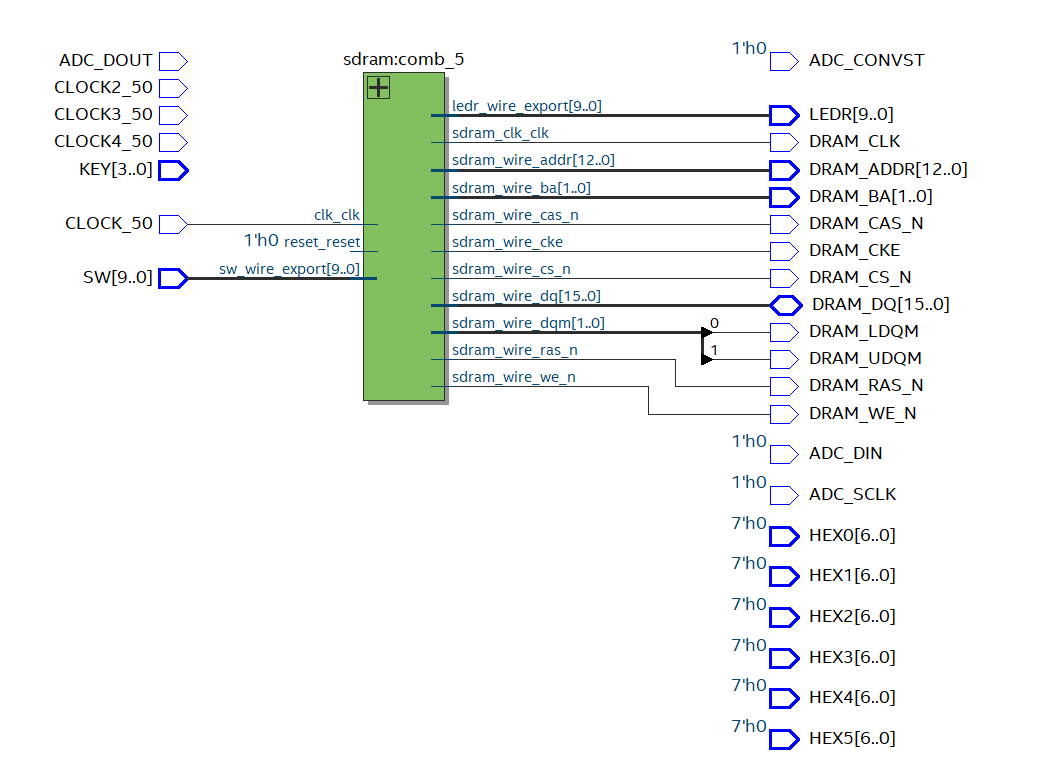
\includegraphics[width=0.9\linewidth]{images/lab45_rtl_view_0.png}
    \caption{RTL View của LAB 4-5}
\end{figure}

\begin{figure}[H]
    \centering
    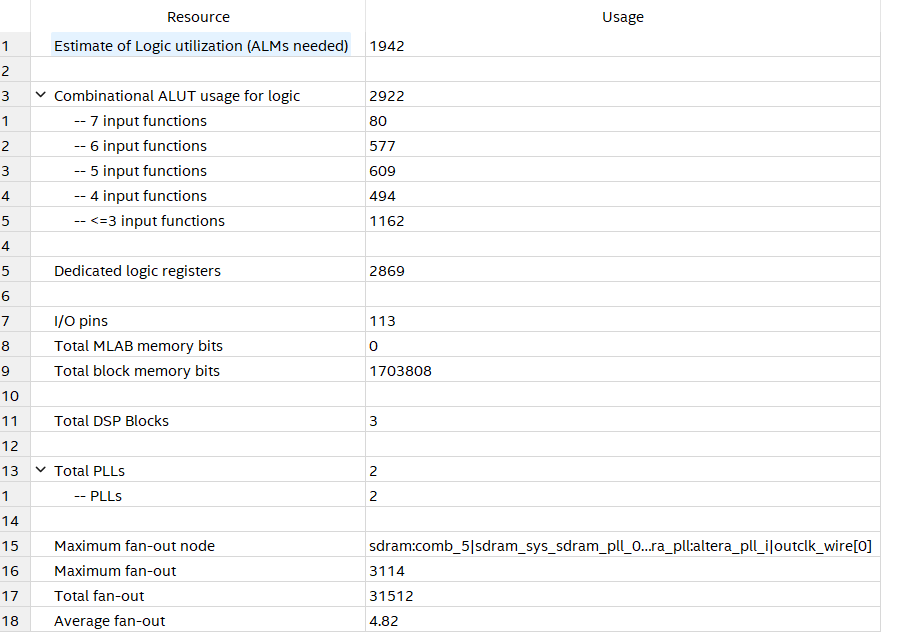
\includegraphics[width=0.9\linewidth]{images/lab45_resource_fmax_0.png}
    \caption{Tài nguyên sử dụng (Resource) của LAB 4-5}
\end{figure}

\begin{figure}[H]
    \centering
    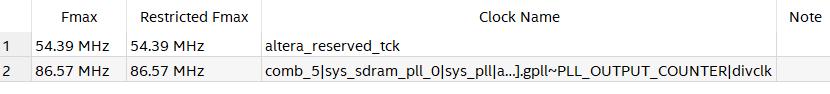
\includegraphics[width=0.9\linewidth]{images/lab45_resource_fmax_1.png}
    \caption{Tần số hoạt động tối đa ($f_{max}$) của LAB 4-5}
\end{figure}

\subsection{Hình ảnh chạy test code trên console}

\noindent\textbf{Video demo (Exercise 1):} \url{Ex1.mp4}

\vspace{0.5cm}

\noindent\textbf{Video demo (Exercise 2):} \url{Ex2.mp4}

\subsubsection*{Kết quả thực thi (Exercise 3)}
\begin{figure}[H]
    \centering
    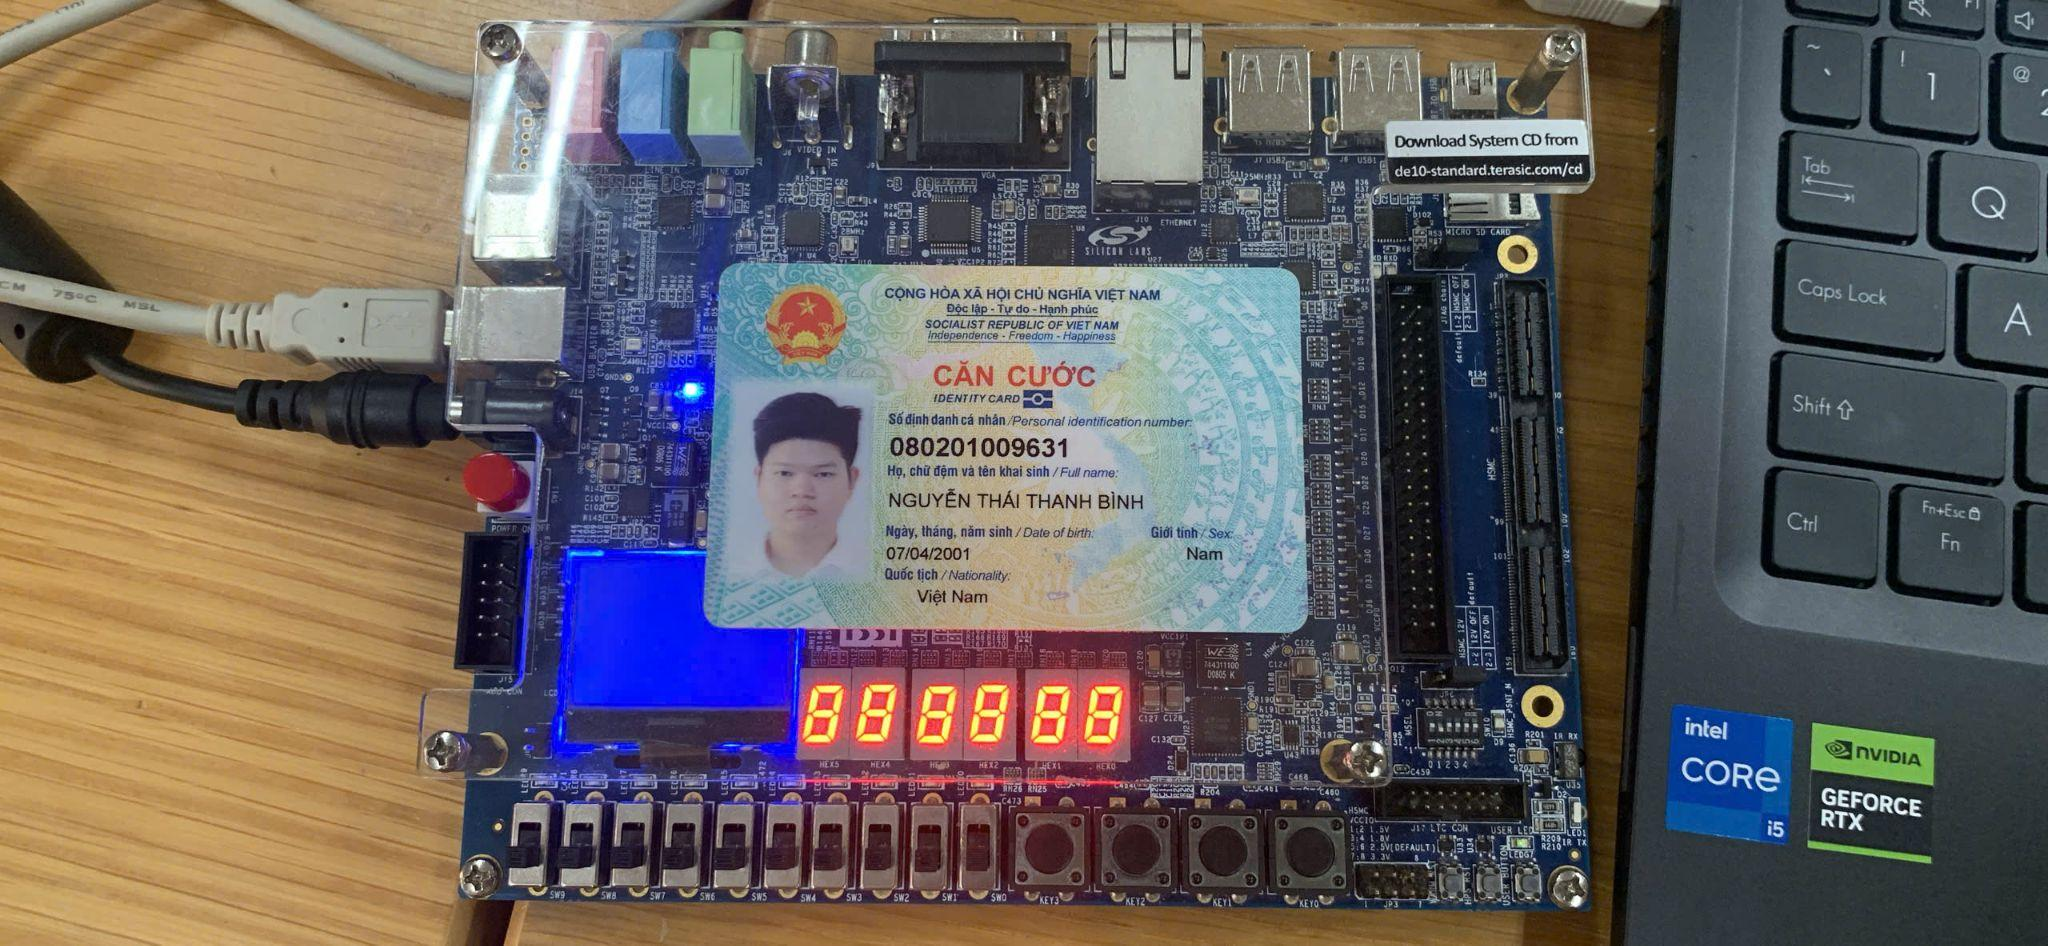
\includegraphics[width=0.8\linewidth]{images/lab45_result_0.jpeg}
    \caption{Kết quả khi cả hai switch đều được thiết lập (Cả 2 switch lên 1)}
\end{figure}

\begin{figure}[H]
    \centering
    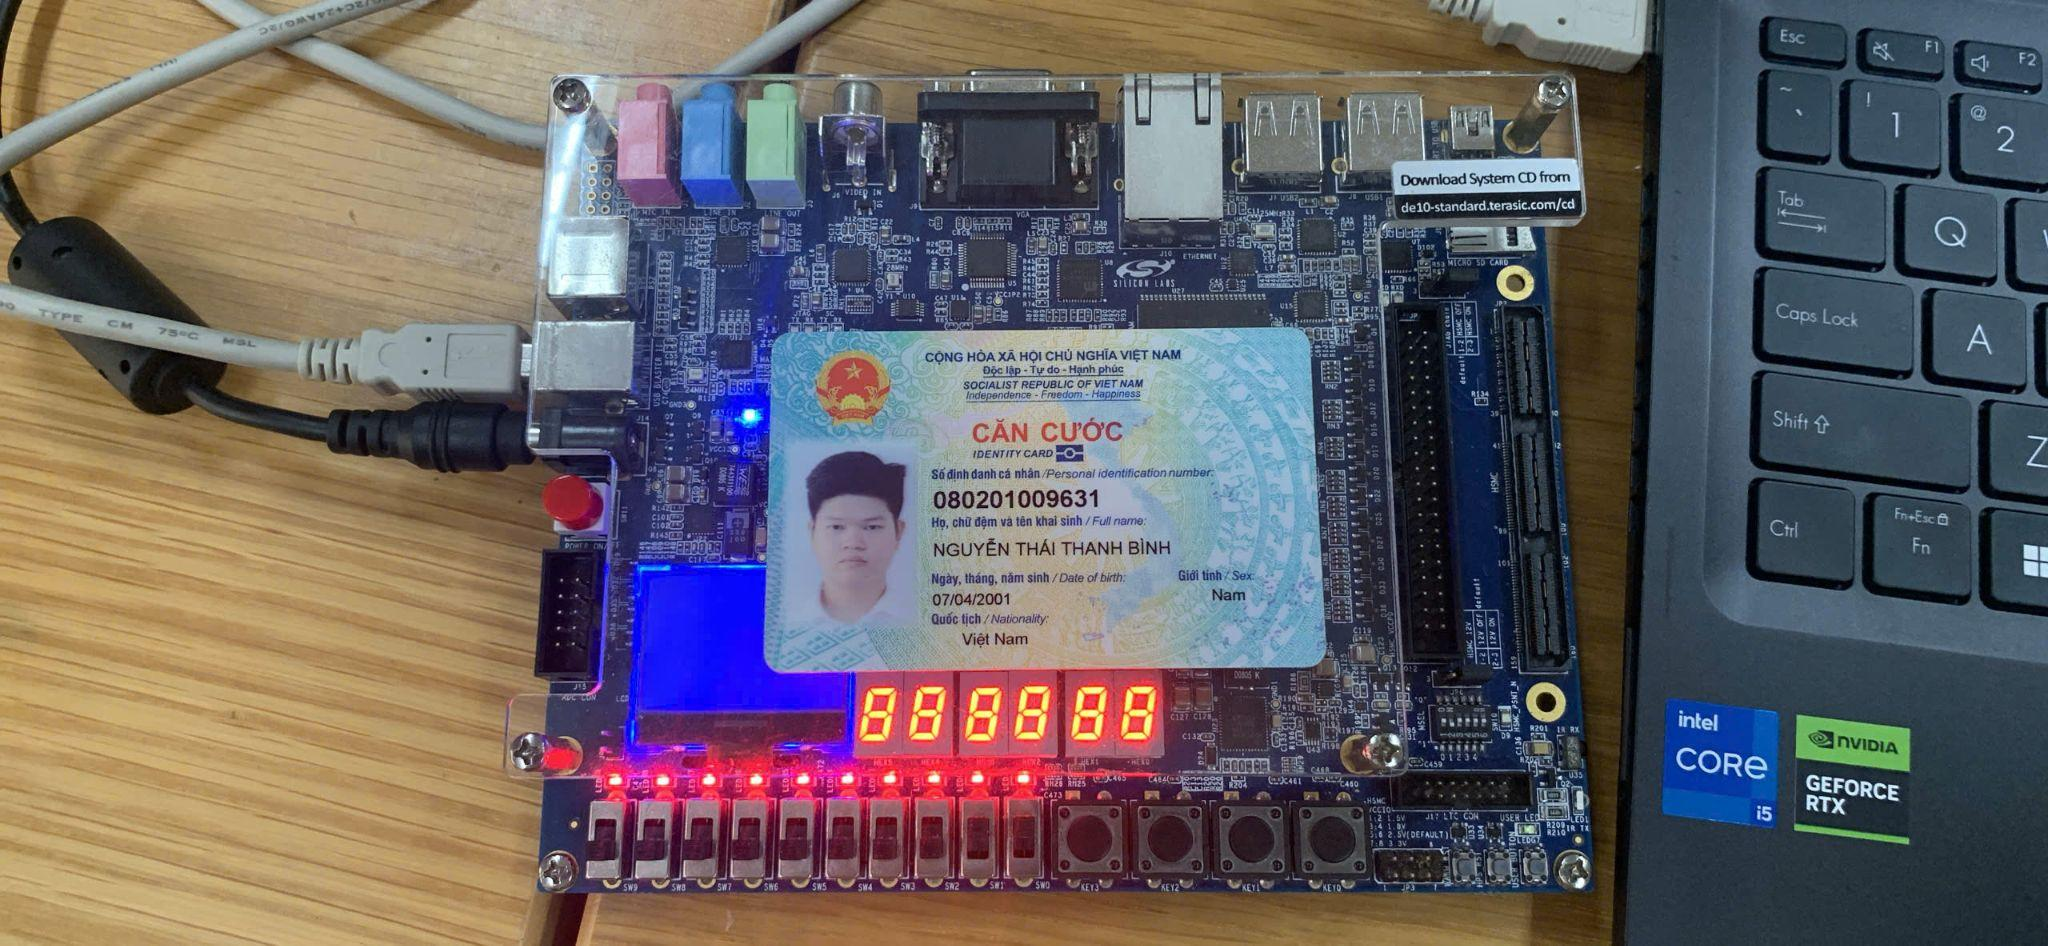
\includegraphics[width=0.8\linewidth]{images/lab45_result_1.jpeg}
    \caption{Kết quả khi cả hai switch đều không được thiết lập (Cả 2 switch về 0)}
\end{figure}

\noindent\textbf{Video demo Switch 1 set (Exercise 3):} \url{Ex3_sw1_set.mp4}

\noindent\textbf{Video demo Switch 2 set (Exercise 3):} \url{Ex3_sw2_set.mp4}

% =========================================================
% LAB 6
% =========================================================
\newpage
\section{LAB6: AVALON MEMORY-MAPPED (AVALON-MM) INTERFACE SPECIFICATION}

\subsection{Trình bày, vẽ sơ đồ mạch theo cách hiểu của học viên}

\textbf{Mục tiêu:} Thiết kế hệ thống Avalon-MM interconnection. Tập trung vào I/O của System Interconnect Fabric, thiết kế Slave Avalon-MM IP (System Interconnect Fabric sẽ tự động kết nối tất cả I/O từ Slave đến Master).

Thêm IP vào dự án Qsys trong Quartus. Sử dụng phần mềm Eclipse để lập trình dự án: Nhân ma trận (Matrix multiplication).

\textbf{Thực hành:} Thiết kế IP thực hiện nhân ma trận sử dụng giao thức Avalon Memory Map. NIOS II được kết nối và sử dụng như một công cụ quản lý dữ liệu, chuyển đầu vào tới và nhận đầu ra từ IP nhân ma trận.

\textbf{Các cổng I/O:}
\begin{itemize}
    \item \textbf{Inputs:} 2 ma trận với các phần tử là số 4-bit.
    \item \textbf{Outputs:} Ma trận chứa kết quả của phép nhân.
\end{itemize}

\begin{figure}[H]
    \centering
    \begin{tikzpicture}[node distance=1.5cm, auto]
        \node[chip, fill=orange!20] (nios) {Nios II Processor (Master)};
        \node[bus, minimum width=8cm, below=of nios] (avalon) {System Interconnect Fabric};
        
        \node[chip, fill=purple!20, below=of avalon] (matrix) {Custom Matrix Multiplication IP\\(Avalon-MM Slave)};
        
        \draw[sarrow, <->] (nios.south) -- (avalon.north -| nios.south);
        \draw[sarrow, <->] (avalon.south -| matrix.north) -- (matrix.north);
        
        \node[block, left=of matrix] (matA) {Matrix A \& B (Inputs)};
        \node[block, right=of matrix] (matRes) {Matrix C (Outputs)};
        
        \draw[signal, ->] (matA.east) -- (matrix.west);
        \draw[signal, ->] (matrix.east) -- (matRes.west);
    \end{tikzpicture}
    \caption{Sơ đồ kiến trúc kết nối IP nhân ma trận thông qua Avalon-MM (LAB 6)}
\end{figure}

\subsection{Sơ đồ dataflow với code software}

\begin{figure}[H]
    \centering
    \begin{tikzpicture}[node distance=0.8cm]
        \node[io] (start) {Bắt đầu chương trình};
        \node[block, below=of start] (gen) {Tạo hai ma trận A, B (4-bit)};
        \node[block, below=of gen] (write) {Ghi ma trận A, B vào Custom IP\\qua Avalon-MM};
        \node[block, below=of write] (wait) {Chờ IP thực hiện nhân ma trận};
        \node[block, below=of wait] (read) {Đọc kết quả ma trận C từ IP};
        \node[block, below=of read] (print) {In ma trận C ra Console};
        \node[io, below=of print] (end) {Kết thúc};
        
        \draw[arrow] (start) -- (gen);
        \draw[arrow] (gen) -- (write);
        \draw[arrow] (write) -- (wait);
        \draw[arrow] (wait) -- (read);
        \draw[arrow] (read) -- (print);
        \draw[arrow] (print) -- (end);
    \end{tikzpicture}
    \caption{Sơ đồ dataflow thuật toán nhân ma trận (LAB 6)}
\end{figure}

Đoạn mã C giao tiếp với Custom IP trên Eclipse:
\begin{lstlisting}[language=C, caption={C Source Code - LAB6 Matrix Multiplication (Ví dụ minh họa)}]
#include <stdio.h>
#include "system.h"
#include "io.h"

// Gia su BASE ADDRESS cua Custom IP la MATRIX_MULT_BASE
#define IP_BASE MATRIX_MULT_BASE

int main() {
    printf("Starting Matrix Multiplication using Custom Avalon-MM IP\n");
    
    // Khoi tao ma tran A va B
    int matrix_a = 0x1234; // Cac phan tu 4-bit
    int matrix_b = 0x5678; 
    
    // Ghi vao Custom IP qua Avalon-MM
    IOWR(IP_BASE, 0, matrix_a);
    IOWR(IP_BASE, 1, matrix_b);
    
    // Bat dau tinh toan
    IOWR(IP_BASE, 2, 0x01); // Ghi co start
    
    // Cho tinh toan xong (gia su thanh ghi 3 la trang thai ready)
    while(IORD(IP_BASE, 3) == 0) {
        // Cho IP tinh xong
    }
    
    // Doc ket qua
    int result = IORD(IP_BASE, 4);
    
    printf("Result Matrix = 0x%X\n", result);
    
    return 0;
}
\end{lstlisting}

\subsection{Báo cáo kết quả Quartus synthesis implementation, resource, $f_{max}$}

\textit{(Sinh viên thay thế các khung trống bên dưới bằng hình chụp kết quả Quartus của LAB 6)}

\begin{figure}[H]
    \centering
    \framebox[\linewidth]{\rule{0pt}{150pt} \Huge \textbf{Ảnh RTL View của LAB 6}}
    \caption{RTL View của Custom Matrix Multiplication IP (LAB 6)}
\end{figure}

\begin{figure}[H]
    \centering
    \framebox[\linewidth]{\rule{0pt}{150pt} \Huge \textbf{Ảnh Resource Usage của LAB 6}}
    \caption{Tài nguyên sử dụng (Resource) của LAB 6}
\end{figure}

\subsection{Hình ảnh chạy test code trên console}

\textit{(Sinh viên thay thế khung trống bên dưới bằng hình chụp kết quả chạy Console của LAB 6)}

\begin{figure}[H]
    \centering
    \framebox[\linewidth]{\rule{0pt}{150pt} \Huge \textbf{Ảnh kết quả Console của LAB 6}}
    \caption{Kết quả chạy test code in ma trận ra console (LAB 6)}
\end{figure}
